\documentclass[conference, italian]{IEEEtran}
\IEEEoverridecommandlockouts
% The preceding line is only needed to identify funding in the first footnote. If that is unneeded, please comment it out.
% \usepackage{cite}
\usepackage{balance}
\usepackage{amsmath,amssymb,amsfonts}
\usepackage{algorithmic}
\usepackage{booktabs}
\usepackage{graphicx}
\usepackage{textcomp}
%\usepackage{biblatex}
\usepackage[natbib=true,backend=bibtex]{biblatex}
\addbibresource{references.bib}
\usepackage{xtab,booktabs}
\usepackage{tabularx}
\usepackage[hidelinks]{hyperref}
\usepackage[italian]{cleveref}
\usepackage[italian]{babel}
\usepackage{listings}
\usepackage{color}
\usepackage[pdftex]{xcolor}
%\usepackage[toc,page]{appendix}

\graphicspath{ {./images/} }

\newcommand\citen[1]{\citeauthor{#1} \citep{#1}}
\newcommand\citetitlen[1]{\citetitle{#1} \citep{#1}}

\def\BibTeX{{\rm B\kern-.05em{\sc i\kern-.025em b}\kern-.08em
    T\kern-.1667em\lower.7ex\hbox{E}\kern-.125emX}}

\definecolor{dkgreen}{rgb}{0,0.6,0}
\definecolor{gray}{rgb}{0.5,0.5,0.5}
\definecolor{mauve}{rgb}{0.58,0,0.82}
\definecolor{backcolour}{rgb}{0.95,0.95,0.92}

\lstdefinelanguage{JavaScript}{
  keywords={typeof, new, true, false, catch, function, return, null, catch, switch, var, if, in, while, do, else, case, break, let, const, for, console},
  keywordstyle=\color{blue}\bfseries,
  ndkeywords={class, export, boolean, throw, implements, import, this},
  ndkeywordstyle=\color{darkgray}\bfseries,
  identifierstyle=\color{black},
  sensitive=false,
  comment=[l]{//},
  morecomment=[s]{/*}{*/},
  commentstyle=\color{purple}\ttfamily,
  stringstyle=\color{red}\ttfamily,
  morestring=[b]',
  morestring=[b]"
}

\lstset{frame=single,
  backgroundcolor=\color{backcolour},
  language=JavaScript,
  aboveskip=3mm,
  belowskip=3mm,
  showstringspaces=false,
  columns=flexible,
  basicstyle={\fontsize{8}{10}\ttfamily},
  numbers=left,
  numberstyle=\tiny\color{black},
  keywordstyle=\color{blue},
  commentstyle=\color{dkgreen},
  stringstyle=\color{mauve},
  breaklines=true,
  breakatwhitespace=true,
  tabsize=3
}

\begin{document}

\title{GPU-based Cryptojacking, attacco e difesa
% {\footnotesize \textsuperscript{*}Note: Sub-titles are not captured in Xplore and
% should not be used}
% \thanks{Identify applicable funding agency here. If none, delete this.}
}

\author{
\IEEEauthorblockN{Anna Lisa Ferrara}
\IEEEauthorblockA{\textit{Dep. of Biosciences and Territory} \\
\textit{University of Molise}\\
annalisa.ferrara@unimol.it}
\and
\IEEEauthorblockN{Federico Zappone}
\IEEEauthorblockA{\textit{Dep. of Biosciences and Territory} \\
\textit{University of Molise}\\
f.zappone1@studenti.unimol.it}
}

\maketitle

\begin{abstract}
In quest'ultimo decennio si è molto discusso di monete digitali e delle così dette criptovalute in seguito all'avvento delle blockchain. Il 3 gennaio 2009 veniva scritto il primo blocco di \emph{Bitcoin}dal valore complessivo inferiore a un dollaro statunitense, in seguito raggiunse il suo massimo storico di quasi \$20.000 ovvero circa 40.000 volte in più. Divenuto un caso più unico che raro, \emph{Bitcoin} si è posto da apripista a più di 5000 altre criptovalute fino ad essere definito come l'oro del \RN{21} secolo, questo grazie anche al processo di creazione delle criptovalute detto \emph{mining}, come nel caso di pietre e metalli preziosi. Grazie alla privacy che queste criptovalute sono in grado di offrire si sono sviluppati diversi tipi di attacchi informatici tra cui il \emph{cryptojacking} in grado di utilizzare potenza computazionale del computer vittima al fine di effettuare \emph{mining} di criptovalute. In questo articolo sarà mostrato in modo concettuale come sarebbe possibile effettuare un attacco di \emph{criptojacking} in combinazione con il \emph{Cross Site Scripting (XSS)} sfruttando inoltre la potenza computazionale della \emph{Graphics processing unit (GPU)} della vittima. \\
\end{abstract}

\begin{IEEEkeywords}
Cryptojacking GPU XSS Injection
\end{IEEEkeywords}

\section{Introduzione}\label{sec:introduction}
In quest'ultimo decennio si è molto discusso di monete digitali e delle così dette criptovalute in seguito all'avvento delle blockchain. Quest'ultima è una tecnologia basata sul concetto di database distribuito, ovvero un sistema che utilizza un registro condiviso per salvare informazioni, esso è modificabile solo dai nodi della stessa rete ed è rappresentabile come una successione di blocchi contenenti delle informazioni. Contemporaneamente alle blockchain è nata anche la prima criptovaluta, più precisamente, il 3 gennaio 2009 veniva scritto il primo blocco di \emph{Bitcoin}~\cite{nakamoto2019bitcoin} dal valore complessivo inferiore a un dollaro statunitense~\citep{kharraz2019outguard}. In seguito il 6 novembre 2010 il valore di \emph{Bitcoin} era di \$0,50, in meno di due anni il prezzo era aumentato di circa 625 volte, e, il 14 aprile 2021, raggiunge il suo massimo storico di circa \$64.800 ~\citep{bitcoinwiki}~\citep{wiredbitcoin}~\citep{coingeckoATH}. Divenuto un caso più unico che raro, \emph{Bitcoin} si è posto da apripista a più di 5000 altre criptovalute~\citep{coinlore} fino ad essere definito come l'oro del \RN{21} secolo. Questa definizione non è dovuta solo all'incredibile aumento del prezzo negli ultimi anni ma anche ad una delle caratteristiche chiave che sia l'oro che la maggior parte delle criptovalute condivide, il processo di ``estrazione'' definito appunto come \emph{mining} nel campo delle monete digitali.\\
Il \emph{mining} di criptovalute consiste nel creare monete virtuali attraverso la risoluzione di alcune funzioni crittografiche necessarie per la validazione delle transazioni e dei blocchi che compongono una blockchain. Questa operazione termina con un compenso da parte della blockchain al \emph{miner}, il quale, avendo offerto la sua potenza di calcolo viene premiato con un compenso monetario. Tali calcoli sono in generale eseguiti da sistemi informatici dedicati a questo specifico processo, essi sono divisi in due macro gruppi in base all'hardware che utilizzano: quelli che sfruttano la Central Processing Unit (CPU) e quelli che sfruttano la \emph{Graphics processing unit (GPU)}. I primi prendono il nome di \emph{ASIC}, acronimo di \emph{Application Specific Integrated Circuit}, ovvero circuiti costruiti per la risoluzione di un calcolo ben specifico che risultano però molto inefficienti su altri tipi di algoritmi. I sistemi basati su GPU sono invece spesso molto più prestanti, le schede video riescono infatti a effettuare più calcoli al secondo rispetto alle CPU che risultano quindi meno redditizie nella maggior parte dei casi di \emph{mining}. D'altro canto per le GPU risulta essere molto più difficile la gestione delle temperature e inoltre comportano costi maggiori sia in termini di assemblaggio che di costi energetici per il mantenimento. Questi ultimi aspetti hanno un notevole impatto per quanto riguarda il \emph{mining}: il costo di acquisto delle componenti è nettamente aumentato negli ultimi anni, sia a causa dell'avanzamento delle tecnologiche più efficienti, sia a causa della grande domanda da parte degli interessati al \emph{mining}.\\
Con l'aumentare dei costi, e allo stesso tempo delle opportunità di guadagno offerte dal mondo in crescita delle blockchain, le criptovalute hanno iniziato a risaltare agli occhi del crimine informatico. Più precisamente la tecnologia blockchain, e di conseguenza una buona parte delle criptovalute, posseggono una caratteristica molto importante per i cyber criminali, ovvero garantiscono una certa forma di anonimato. Le criptovalute infatti sono difficilmente riconducibili ad una persona fisica diversamente da un conto bancario classico. Le criptovalute sono infatti collegare ad un portafoglio digitale, detto appunto \emph{wallet}. L'accesso ai \emph{wallets} non è però regolamentato, e quindi non collegato fisicamente a qualcuno. Questa caratteristica ha portato a un enorme utilizzo delle criptovalute per lo svolgimento di azioni illecite, nel 2017 infatti si è riscontrato un netto aumento dei così detti \emph{ransomware}~\citep{skyboxtrends}, ovvero virus che una volta bloccato il sistema sul quale sono eseguiti chiedono un riscatto per il suo sblocco. Tale pagamento di tale riscatto è richiesto sotto forma di criptovalute per mantenere l'anonimato. Successivamente si è arrivati a una forma di attacco più ``intelligente'' e meno invasiva, ovvero i \emph{cryptominers}. Definito appunto come ``l'anno dei cryptominers'', il 2018 vede la stessa impennata di casi di \emph{ransomware} dell'anno precedente sotto una nuova forma di attacco che consiste nell'utilizzare potenza computazionale della vittima per generare criptovalute ~\ref{fig:topmalwarefamilies}. Il tutto avviene seguendo un basso profilo, tramite programmi infetti che vengono installati sul computer o, come più recentemente si è affermato, attraverso script malevoli presenti all'interno di pagine web comuni. La differenza tra l'utilizzo di programmi eseguibili e gli script presenti online sta principalmente nella loro rintracciabilità e facilità di utilizzo, infatti quelli che operano attraverso il web sono più difficili da individuare e analizzare rispetto a programmi che devono necessariamente essere installati dall'utente e che, quindi, sono sotto l'occhio diretto di antivirus e delle politiche dettate dal sistema operativo.\\
L'utilizzo della GPU in all'interno di browser è ad oggi possibile, anche se non largamente diffuso, tramite l'utilizzo di alcune librerie e specifiche web. \citetitle{OpenGL} (\emph{Open Graphics Library}) è considerata ormai lo standard per quanto riguarda la grafica tridimensionale in sistemi operativi \emph{Unix-like}, in particolare, essa è stata pensata per architetture parallelizzabili come le GPU e definisce delle \emph{API} per applicazioni che operano in ambienti 3D.\ Su questo standard sono basate altre librerie che permettono l'utilizzo della GPU in ambito web come \citetitle{WebGL}. Quest'ultima è una \emph{Web-based Graphics Library} ovvero una libreria pensata per la gestione di elementi grafici all'interno del web, essa fornisce delle \emph{API} per grafica 3D in un contesto \emph{HTML5} tramite l'utilizzo del \emph{Document Object Model (DOM)}. Da \citetitle{WebGL} si arriva poi a \citetitle{GPU.js}, ovvero una libreria implementata interamente attraverso il linguaggio \emph{JavaScript} e pensata per sfruttare l'accelerazione hardware delle GPU attraverso l'utilizzo del medesimo linguaggio.\\
L'utilizzo di un linguaggio di scripting web come \emph{Javascript} è a sua volta rilevante in quanto esso può essere utilizzato per portare a termine attacchi che sfruttano vulnerabilità di tipo \emph{Cross Site Scripting (XSS)}. Gli attacchi di tipo \emph{XSS} sono tra i più diffusi all'interno del web, infatti, secondo il report di \citen{PositiveTechnologiesReport}, la percentuale di questi attacchi è salita dall'occupare il 77,9\% nel 2017 all'88,5\% di tutte le tipologie di attacchi web registrate nel 2018. Secondo \citen{PreciseSecurityReport} invece, in rapporto a tutti i tipi di attacchi sferrati verso le grandi compagnie di Europa e Nord America nel 2019, la percentuale di attacchi di \emph{Cross Site Scripting} risulta essere del 39\%, superando più del doppio la percentuale degli attacchi di \emph{SQL Injection}.\\
L'\emph{XSS} consiste nell’introdurre del codice arbitrario lato client all'interno dei siti web con il fine di eseguire una serie di attacchi rivolti ai visitatori. Questa vulnerabilità affligge i siti dinamici che non effettuano un controllo sugli input lato client, il che porta ad una ``fusione'' tra il payload, ovvero il codice inserito dall'attaccante, e il codice reale della pagina. Questa tipologia di attacchi si suddivide a sua volta in tre gruppi:
\begin{itemize}
  \item XSS reflected: il payload viene eseguito solo nel momento dell’iniezione;
  \item XSS stored: il payload viene salvato all'interno della struttura dell'applicativo ed eseguito ad ogni accesso del contenuto;
  \item XSS DOM-based: il codice sorgente e la risposta del server non vengono modificate, il payload viene eseguito a runtime senza inoltrare richieste al server ma utilizzando il codice già presente nella pagina.
\end{itemize}
Esistono vari strumenti in grado di analizzare la struttura delle pagine web e di identificare vulnerabilità \emph{XSS}, come ad esempio \citetitlen{XSStrike}, \citetitlen{Traxss} e \citetitlen{XSSer}. Questi sono tutti tool open-source di analisi sviluppati in \emph{Python}, il più interessante è però \citetitle{XSSer}, uno dei tool preinstallati presenti nelle distribuzioni \emph{Linux} atte al \emph{penetration testing}. Si è quindi pensato di utilizzare uno di questi tool per individuare in modo semi-automatico o del tutto automatico le vulnerabilità \emph{XSS} all'interno di siti web.

\subsection{Obiettivi e struttura dell'articolo}\label{subsec:objectives-and-article-structure}
L'obiettivo principale di questo articolo è quindi quello di mostrare come sia possibile effettuare un attacco di tipo \emph{cryptojacking} basato sfruttando la potenza computazionale della GPU della vittima, il tutto applicato in un contesto web. Inoltre una volta mostrato il vettore di attacco saranno mostrate le debolezze e da in seguito a queste anche una possibile difesa.\\
Il resto dell'articolo è strutturato nel modo seguente:
\cref{sec:related-work} introduce quello che è lo stato dell'arte per quanto riguarda gli attacchi \emph{cryptojacking},
\cref{sec:gpu-web-based-cryptominer} descrive come è possibile utilizzare la GPU in un contesto web,
\cref{sec:cryptominer-automatic-injection} mostra l'injection automatizzata del payload,
\cref{sec:testing-environment} descrive le caratteristiche dell'ambiente di test utilizzato,
\cref{sec:non-invasive-defence} individua una soluzione difensiva user-friendly,
\cref{sec:results} analizza i risultati ottenuti,
\cref{sec:conclusion} conclude e riassume l'articolo ed infine
\cref{sec:future-works} identifica quelli che sono le azioni future che saranno effettuate.


\begin{figure*}[hbt!]
\centering
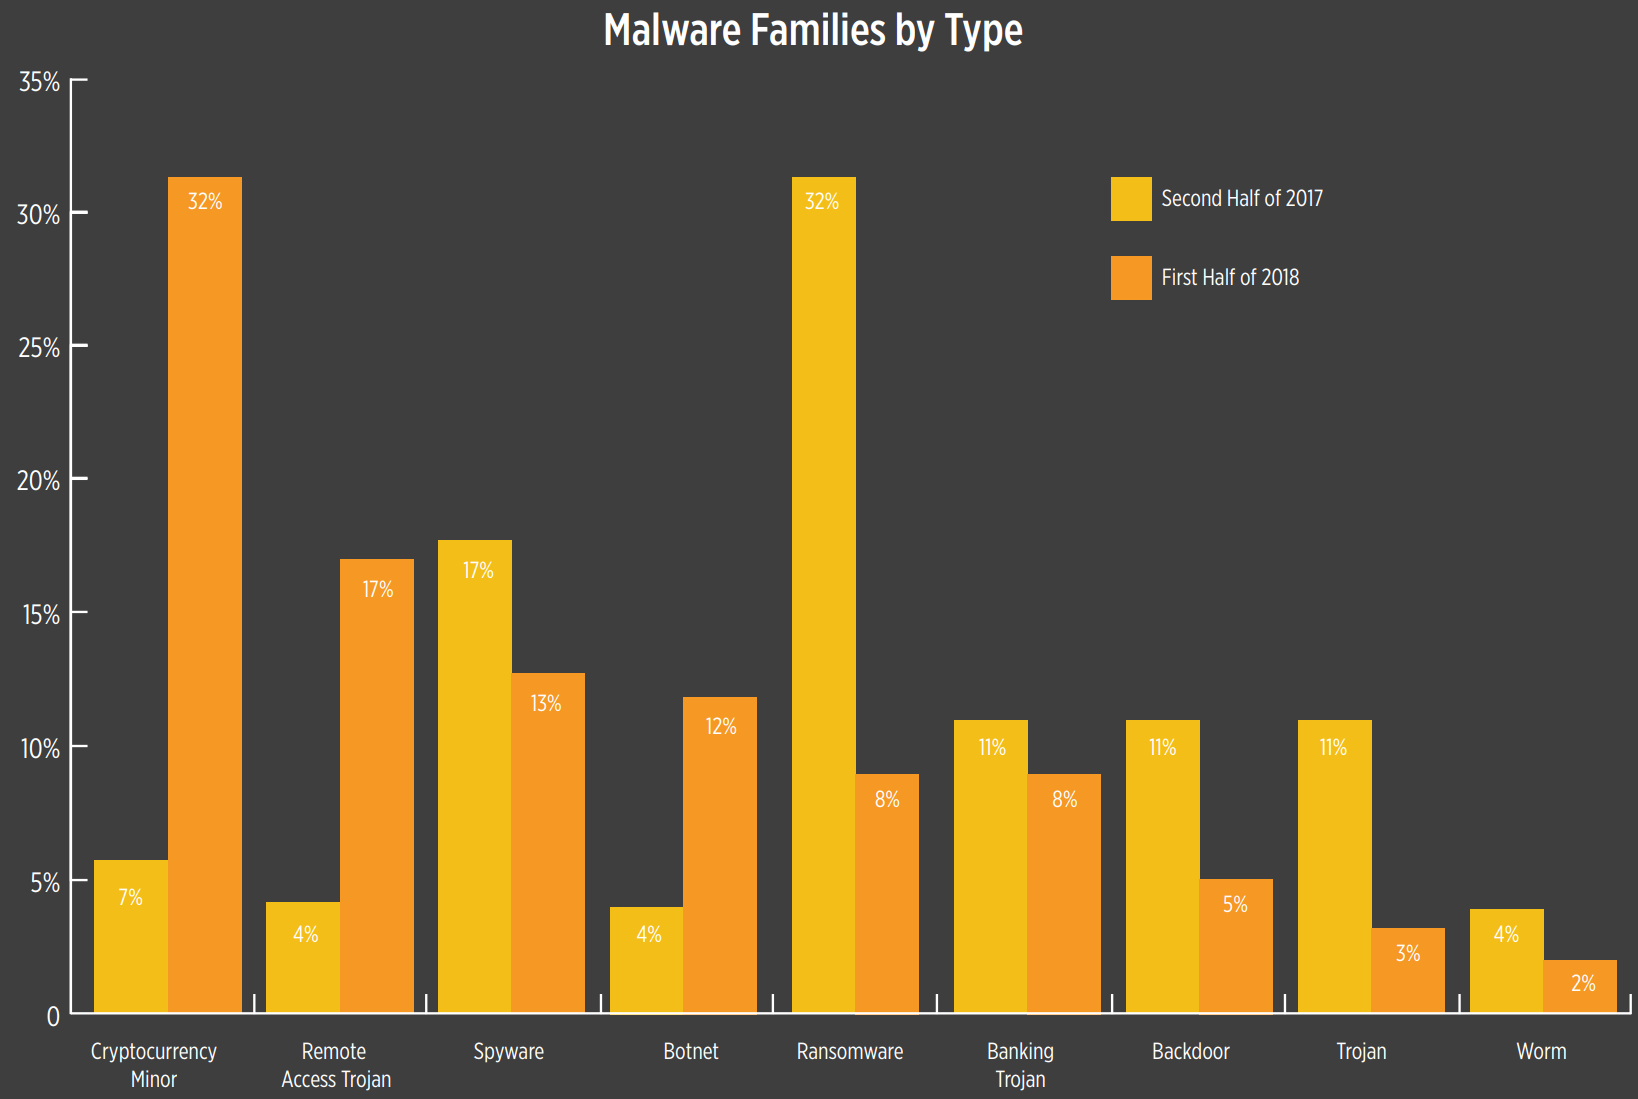
\includegraphics[width=0.8\textwidth]{TopMalwareFamilies.png}
\caption{Top Malware Families by type, 2018, \citetitlen{skyboxtrends}}\label{fig:topmalwarefamilies}
\end{figure*}


\section{Stato dell'arte}\label{sec:related-work}
Le GPU grazie alla loro potenza offrono quindi nella maggior parte dei casi dei ricavi maggiori nel \emph{mining} rispetto alle CPU, di contro però non sono facilmente utilizzabili in ambito web. Ciò ha portato infatti ad uno sviluppo maggiore dei \emph{cryptominers} basati su CPU e, di conseguenza, a sistemi di difesa che si concentrano su di essi. \citen{musch2018web} e \citen{saad2018end} mostrano la diffusione dei \emph{cryptominers} basati su CPU all'interno del web, inoltre analizzano l'efficacia di tecniche difensive di blacklisting che risultano però essere una protezione non sempre efficiente sebbene pratica. \citen{wang2018seismic} mostra in seguito un metodo di analisi di firme basate su istruzioni della CPU durante l'esecuzione dei moduli \emph{WebAssembly}. \citen{konoth2018minesweeper} introduce invece \emph{MineSweeper} basato anch'esso sul principio di firme ma con l'aggiunta del rilevamento di eccessive chiamate di sistema di natura crittografica legate agli algoritmi di mining durante l'esecuzione di un programma. \citen{kharraz2019outguard} dimostra invece che come l'analisi della CPU generi una grande quantità di falsi positivi all'interno della navigazione web. Un differente approccio viene fornito da \citen{tahir2017mining} che presenta \emph{MineGuard}, un sistema che tramite l'analisi delle prestazioni hardware rileva l'esecuzione di alcuni algoritmi di \emph{mining}. \emph{MineGuard} monitora costantemente l'hardware del computer e inoltre offre un'ottima soluzione sia in termini di efficienza che di utilizzo di risorse per la sua esecuzione. \citen{belkin2019risks} offre infine una soluzione dedicata esclusivamente a \emph{cryptominers} di GPU che risulta essere decisamente più pratica in ambito web rispetto alle altre, andando a limitare le pagine web che utilizzano \citetitlen{WebGL}.

\section{Metodologie utilizzate}\label{sec:methodologies}
\subsection{GPU-WEB based Cryptominer}\label{sec:gpu-web-based-cryptominer}
L'utilizzo di \emph{Graphics processing units} all'interno di pagine web non è molto comune nonostante negli ultimi anni sia nettamente aumentata la complessità degli elementi grafici presenti all'interno dei browser. Ciononostante sono state sviluppate delle \emph{Application Programming Interface} per garantire l'operabilità di processori grafici in un contesto web. In particolare ciò è reso possibile da \citetitle{OpenGL} che a sua volta è utilizzato da librerie come \citetitle{WebGL} e \citetitle{GPU.js}. In particolare, \citetitle{GPU.js} è pensata per computare fino a quindici volte più rapidamente della sola CPU operazioni parallelizzabili come il caricamento di elementi grafici complessi o la moltiplicazione di matrici di grandi dimensioni~\citep{banchmarkGPU.js}. Operando in un contesto di grafica tridimensionale, queste implementazioni permettono di effettuare operazioni anche complesse attraverso la GPU dell'utente che visualizza la pagina web dove sono utilizzate. L'idea è quindi quella di sviluppare un \emph{cryptominer} attraverso l'utilizzo di queste librerie. In particolare si è scelto di utilizzare \emph{GPU.js} per lo sviluppo del payload malevolo in quanto si presta bene all'injection in quanto l'implementazione avviene attraverso il linguaggio \emph{Javascript}. Unico svantaggio dell'utilizzo di librerie grafiche è il fatto che non permettono di eseguire qualsiasi tipo di operazioni, infatti, non è prevista la possibilità di effettuare \emph{HTTP requests}. Ciò costituisce una grande limitazione quando si tratta di operazioni che necessitano costantemente di dati esterni alla pagina web per l'esecuzione. Questa limitazione rende infatti problematico il collegamento con le blockchain e di conseguenza il mining di criptovalute. Sarebbe comunque possibile effettuare mining attraverso \emph{GPU.js} nel caso in cui vi sia una re-implementazione dello \emph{Stratum protocol} \cite{recabarren2017hardening} utilizzato per il dialogo con le pool di mining e le blockchain. Pertanto nel corso di questo articolo è stato utilizzato come payload ``malevolo'' uno script che permette l'utilizzo della GPU per il calcolo di due matrici quadrate di dimensione 8096 righe e colonne composte da valori generati in modo casuale. Lo script prevede inoltre l'importazione dinamica della libreria GPU.js e l'avvio automatico delle operazioni di calcolo \cref{appendix:gpu-payload}.

\subsection{Cryptominer injection automatizzata}\label{sec:cryptominer-automatic-injection}
Come precedentemente si è detto nella \cref{sec:gpu-web-based-cryptominer}, l'utilizzo della libreria \emph{GPU.js}, e in particolare del linguaggio \emph{JavaScript}, non è dovuta solo al fatto che è uno dei più utilizzati e supportati all'interno del web \citep{w3techsJavascriptPopularity}, ma soprattutto al fatto che è tra i principali utilizzati per l'iniezione di codice malevolo. Spesso infatti gli attacchi di tipo \emph{XSS} sono portati a termine tramite iniezione di codice \emph{Javascript} ~\citen{owaspxss}.\\
Per l'effettiva esecuzione dell'attacco si è sviluppato un tool di injection automatica in linguaggio \emph{BASH} e basato sul software \emph{XSSer}. Il tool sviluppato è basato su un file descrittore \cref{appendix:descriptor-file} nel quale sono presenti le informazioni relative alle modalità di scansione e di attacco. Il tool prevede cinque modalità principali:
\begin{itemize}
  \item GET, utilizzata per \emph{HTTP requests} di tipo ``GET'';\@
  \item POST, utilizzata per \emph{HTTP requests} di tipo ``POST'';\@
  \item ALL, utilizzata per vettori di attacchi su tutto il sito vittima;
  \item AUTO, automatica che utilizza delle euristiche;
  \item DEFAULT, standard molto simile alla modalità ALL.\@
\end{itemize}
Oltre alla definizione della modalità di scanning e di attacco è necessario definire l'endpoint e i parametri necessari per le chiamate di tipo ``GET'', analogamente per le chiamate ``POST'', ponendo attenzione nell'inserire in entrambi i casi il placeholder ``XSS'' al posto di almeno un valore. Il placeholder sarà poi riconosciuto dal tool e, durante l'esecuzione, sarà rimpiazzato con i payload di scan e infine il payload di attacco. Vi è inoltre la possibilità di definire i \emph{cookies} di sessione necessari per la corretta esecuzione su alcune applicazioni web. I \emph{cookie} possono essere inseriti nella colonna finale del file descrittore e saranno poi automaticamente gestiti dal tool durante le varie fasi.
L'esecuzione del tool può essere inoltre lanciata secondo due sotto-modalità ovvero scanning e injection. Le sotto-modalità sono indipendenti tra loro, infatti esse sono utilizzabili sia singolarmente che in combinazione. Infine, In entrambi i casi è possibile definire un payload personalizzato, in caso di scansione sarà utilizzato per ricercare vulnerabilità mentre in caso di injection sarà invece iniettato seguendo i vettori di attacco precedentemente individuati. Le modalità precedentemente descritte sono effettuate operando in \emph{multithread}, per velocizzare l'esecuzione e utilizzando un \emph{fake user-agent} con l'intento di oltrepassare i controlli e le limitazioni di accesso ripetuto per la maggior parte dei siti web.\\
Il tool in seguito all'esecuzione dello scanning di vulnerabilità genera un file di report al quale viene associato un controllo di integrità. Il report contiene tutti i test e i vettori di attacco analizzati e le informazioni riguardanti quali il risultato dell'operazione e una lista di attacchi andati a buon fine qualora ce ne siano. Il file di report viene infine consultato in fase di attacco per determinare il vettore di attacco con accuratezza più elevata e sfruttarlo per iniettare il payload malevolo.\\
Come mostrato in \cref{appendix:injected-payload} il payload finale non coincide esattamente con il payload contenente le operazioni computazionali complesse, bensì consiste nell'iniezione di un tag ``<script>'' avente come sorgente un \emph{endpoint} che fornirà integralmente lo script. Questo processo è essenziale in quanto si vogliono evitare limitazioni sul numero di caratteri inserendo così un payload di dimensioni contenute che però sortirà lo stesso effetto rispetto al payload malevolo basato su \emph{GPU.js}.

\subsection{Testing environment}\label{sec:testing-environment}
L'ambiente sul quale si sono effettuati i test di validazione dell'attacco è stato creato appositamente utilizzando \emph{Damn Vulnerable Web App (DVWA)}\cite{DVWA}. Quest'ultima è un'applicazione web codificata utilizzando \emph{PHP} e \emph{MySQL} il quale obiettivo principale è quello di creare un ambiente appositamente vulnerabile ma controllato che permetta lo studio delle problematiche di sicurezza più frequenti in ambito web e che divide le vulnerabilità in tre diverse difficoltà.\\
Al fine di ridurre al minimo le possibilità di danneggiamento del sistema in uso, e soprattutto per permettere la riproducibilità dell'attacco, l'applicativo \emph{DVWA} è stato eseguito all'interno di un sistema di ``containerizzazione'' quale \emph{Docker}\cite{merkel2014docker}. Il container è stato predisposto per essere facilmente ricreato ed è inoltre stato aggiunto il supporto all'utilizzo della utility \emph{docker-compose} per una ancor più facile interazione con il container di test.
Infine è stato sviluppato un applicativo server con lo scopo di fungere da \emph{dispatcher} per quanto riguarda il payload malevolo. Il server è stato realizzato in \emph{Python} nella sua terza versione\cite{python3} e in particolare con il framework \emph{Flask}\cite{grinberg2018flask}. Il \emph{dispatcher} sviluppato ha il solo scopo di simulare il server dell'attaccante o un qualsivoglia fornitore di un servizio capace di fornire su richiesta il payload malevolo con \emph{MIME Type: text/javascript}\cite{MIMEType}.

\subsection{Soluzione difensiva non invasiva}\label{sec:non-invasive-defence}
Analizzando i risultati ottenuti da~\citen{wang2018seismic} una tecnica difensiva molto efficace consiste nel monitorare costantemente l'utilizzo dell'hardware del computer vittima per individuare l'attacco e interrompere il processo di esecuzione. Nonostante il \emph{monitoring} della componentistica possa essere ridotto al riconoscimento delle sole funzioni crittografiche, come mostrato da~\citen{konoth2018minesweeper}, un approccio di questo tipo risulta essere sì efficace ma anche invasivo e richiede la continua esecuzione del processo di controllo in background con conseguente utilizzo di risorse.\\
Un approccio più \emph{user-friendly} è invece quello individuato da~\citen{belkin2019risks}, ovvero analizzare durante la navigazione web se si utilizzano funzioni e librerie grafiche pensate per GPU e bloccarne l'esecuzione. Questa tecnica difensiva seppur ``semplice'' offre molti vantaggi, primo tra tutti risolve il problema della \emph{code obfuscation} in quanto non analizza il codice eseguito direttamente, che potrebbe essere offuscato, ma solo l'accesso alle librerie web che sono richieste dalla pagina. Pertanto è stata impostata una tecnica difensiva basata sul blocco di quelle librerie web che permettono l'utilizzo di processori grafici. Il risultato di tale operazione è stato lo sviluppo di un'estensione web per il browser \emph{Google Chrome} che neutralizza l'utilizzo della libreria \emph{GPU.js} bloccando la richiesta di download del codice malevolo sul nascere. È importante far notare che la scelta di un'estensione è stata presa considerando anche la facilità di utilizzo da parte di un utente inesperto, infatti, le estensioni dei browser permettono lo sviluppo di interfacce semplici da utilizzare per l'utente e che permettono la personalizzazione di operazioni come il blocco dell'estensione solo su determinati siti o l'aggiunta di ulteriori librerie considerate non affidabili, così da garantire una maggiore personalizzazione e scalabilità.


\section{Analisi dei risultati e implementazioni future}\label{sec:results-analysis}
\subsection{Risultati}\label{sec:results}
I test effettuati si sono svolti andando ad utilizzare il tool di analisi e di attacco sviluppato impostando come target le pagine vulnerabili esposte da \emph{DVWA}. Nel dettaglio ci si è concentrati sulle vulnerabilità di tipo \emph{XSS stored} in quanto esse erano quelle più interessanti per questo tipo di attacco in un contesto reale. Il tool ha portato al corretto sfruttamento delle vulnerabilità in tutti e tre i livelli di difficoltà proposti da \emph{DVWA}.\\
Una volta provata l'efficacia dell'attacco si è testata anche l'efficacia del sistema di difesa che è correttamente riuscito a bloccare l'utilizzo della libreria \emph{GPU.js}. Il blocco della libreria è stato prontamente rilevato ad ogni caricamento della pagina ed è stata correttamente bloccata l'esecuzione dello script precedentemente iniettato.
Possiamo quindi affermare che i risultati ottenuti siano stati soddisfacenti per quanto riguarda l'attacco dal punto di vista concettuale in quanto si è dimostrato che questo approccio è effettivamente utilizzabile e che è anche in qualche modo neutralizzabile.

\subsection{Conclusione}\label{sec:conclusion}
In quest'ultimo decennio si è molto discusso di monete digitali e delle così dette criptovalute in seguito all'avvento delle blockchain. In seguito l'interesse dalle criptovalute si è espanso fino a generare un grande interesse per le tecniche di \emph{mining} con le quali le \emph{cryptocurrencies} vengono generate. Di conseguenza il \emph{mining} è diventato di grande interesse anche per i malintenzionati portando allo sviluppo di attacchi di basso profilo di \emph{cryptojacking}.\\
In questo articolo è stato mostrato come sia possibile effettuare un attacco di \emph{cryptojacking} che utilizzi la potenza della \emph{Graphics processing unit} all'interno del browser web. Nonostante il \emph{cryptominer} ideato non sia stato completato a causa delle limitazioni delle tecniche utilizzate, il payload di test dimostra comunque la fattibilità di esecuzione dell'attacco basato su GPU.\@ Si è inoltre sviluppato un tool di injection automatica del payload malevolo tramite attacchi di tipo \emph{Cross Site Scripting}, la cui bontà è stata testata all'interno di un ambiente \emph{Docker} contenente un'istanza di \emph{Damn Vulnerable Web App}. Il testing ha prodotto risultati soddisfacenti riuscendo ad analizzare, individuare e sfruttare le vulnerabilità presenti nelle tre diverse difficoltà. In seguito si è sviluppato un sistema di difesa \emph{user-friendly} pensato per l'utilizzo comune di utenti inesperti ma comunque attento alle loro esigenze di personalizzazione.

\subsection{Sviluppi futuri}\label{sec:future-works}
Il prossimo passo per il completamento effettivo dell'attacco sarà quello di integrare lo \emph{Stratum Protocol} all'interno del payload malevolo da iniettare all'interno dei siti target. In questo modo si potrà inoltre confrontare il \emph{mining} tramite browser e quello classico così da studiarne i pro e i contro. Ciò oltre ad offrire un metodo di paragone tra le due modalità potrebbe portare ad un nuovo tipo di mining nel caso in cui le prestazioni siano simili. Se le due modalità si rivelassero equivalenti si potrebbe infatti semplificare l'accesso al mondo del \emph{mining} che potrebbe essere effettuato semplicemente navigando ad un indirizzo web.\\
Infine una ulteriore miglioria potrebbe essere quella di permettere una maggiore personalizzazione e l'implementazione di una grafica minimalista per quanto riguarda l'estensione di difesa contro questo tipo di attacchi. In questo modo si avrebbe un prodotto finito e accessibile agli utenti inesperti che potrebbe essere integrato come controllo durante la navigazione.

\balance
\newpage
\printbibliography
\vspace{12pt}


\onecolumn
\begin{appendices}
\appendix
  \section*{GPU.js payload}\label{appendix:gpu-payload}
  \lstinputlisting[language=JavaScript, numbers=left,xleftmargin=3em]{code/gpu-payload.js}

  \section*{Injected payload}\label{appendix:injected-payload}
  \lstinputlisting[language=JavaScript, numbers=left,xleftmargin=3em]{code/inject-payload.js}

  \section*{Esempio file descrittore}\label{appendix:descriptor-file}
  \lstinputlisting[numbers=left,xleftmargin=3em]{code/sites-urls.txt}
\end{appendices}

\end{document}
